% Emerald Publishing - Construction Innovation Submission Template
% by Oleksandr Melnyk
% Ver 0.0.4
% Based on: https://www.emeraldgrouppublishing.com/journal/ci#author-guidelines


\documentclass{article}

\usepackage[english]{babel}

% Set page size and margins
% Replace `letterpaper' with `a4paper' for UK/EU standard size
\usepackage[letterpaper,top=2cm,bottom=2cm,left=3cm,right=3cm,marginparwidth=1.75cm]{geometry}

% Useful packages
\usepackage{amssymb}
\usepackage{siunitx}
\PassOptionsToPackage{hyphens}{url}\usepackage{hyperref}
\usepackage{cleveref}
\usepackage[utf8]{inputenc}
\usepackage[right]{lineno}
\usepackage{csquotes}
\usepackage{booktabs}
\usepackage{subcaption}
\usepackage{longtable}
\usepackage{adjustbox}
\usepackage{multirow}
\usepackage{array}
\usepackage{url}
\usepackage{titlesec}
%\usepackage[compatibility=false]{caption}
\usepackage{authblk}
\usepackage{xcolor} % Load the xcolor package for color options
\renewcommand{\thetable}{\Roman{table}}
\usepackage{tabularx}
% Define a new format for \subsection
\titleformat{\subsection}
  {\mdseries\itshape\large} % Medium series, italic shape, and large font size
  {\thesubsection}{1em}{} % Numbering, spacing, and the section title itself


% Emerald Harvard Citation Style

\usepackage[english]{babel}
\usepackage[style=authoryear,backend=biber,natbib=true,maxcitenames=2,uniquelist=false]{biblatex}
\addbibresource{Bibliography.bib} % your .bib file

% Customizing biblatex for Harvard style
% Customizing biblatex for Harvard style
\DeclareNameAlias{sortname}{family-given}
\DeclareNameAlias{default}{family-given}

\renewbibmacro{in:}{}
\DeclareFieldFormat[article]{title}{\mkbibquote{#1}\addcomma}
\DeclareFieldFormat[book]{title}{\mkbibemph{#1}\addcomma}
\DeclareFieldFormat[bookinbook]{title}{\mkbibemph{#1}\addcomma}
\DeclareFieldFormat[inbook]{title}{\mkbibquote{#1}\addcomma}
\DeclareFieldFormat[incollection]{title}{\mkbibquote{#1}\addcomma}
\DeclareFieldFormat[inproceedings]{title}{\mkbibquote{#1}\addcomma}
\DeclareFieldFormat[manual]{title}{\mkbibemph{#1}\addcomma}
\DeclareFieldFormat[misc]{title}{\mkbibemph{#1}\addcomma}
\DeclareFieldFormat[thesis]{title}{\mkbibemph{#1}\addcomma}
\DeclareFieldFormat[unpublished]{title}{\mkbibquote{#1}\addcomma}
\DeclareFieldFormat[patent]{title}{\mkbibemph{#1}\addcomma}
\DeclareFieldFormat[report]{title}{\mkbibemph{#1}\addcomma}
\DeclareFieldFormat[online]{title}{\mkbibquote{#1}\addcomma}
\DeclareFieldFormat[software]{title}{\mkbibemph{#1}\addcomma}
\DeclareFieldFormat[booklet]{title}{\mkbibemph{#1}\addcomma}
\DeclareFieldFormat[periodical]{title}{\mkbibemph{#1}\addcomma}
\DeclareFieldFormat[standard]{title}{\mkbibemph{#1}\addcomma}

\DeclareFieldFormat[article]{journaltitle}{\iffieldundef{shortjournal}{\mkbibemph{#1}\addcomma}{\mkbibemph{\printfield{shortjournal}}\addcomma}}
\DeclareFieldFormat{volume}{\bibstring{volume}~#1}
\DeclareFieldFormat{number}{\bibstring{number}~#1}

% Definitions for "Vol." and "No."
\DefineBibliographyStrings{english}{
  volume = {Vol.},
  number = {No.}
}

\renewbibmacro*{volume+number+eid}{%
  \printfield{volume}%
  \setunit*{\addspace}%
  \printfield{number}%
  \setunit{\addcomma\space}%
  \printfield{eid}}

\renewbibmacro*{journal+issuetitle}{%
  \usebibmacro{journal}%
  \setunit*{\addcomma\space}%
  \usebibmacro{volume+number+eid}%
  \setunit{\addcomma\space}%
  \usebibmacro{issue+date}}

\renewbibmacro*{publisher+location+date}{%
  \printlist{publisher}%
  \iflistundef{location}
    {\setunit*{\addcomma\space}}
    {\setunit*{\addcolon\space}}%
  \printlist{location}%
  \setunit*{\addcomma\space}%
  \usebibmacro{date}}

\renewcommand*{\bibpagespunct}{\addcomma\space}

% Customizing citations for Harvard style
\DeclareCiteCommand{\cite}[\mkbibparens]
  {\usebibmacro{prenote}}
  {\usebibmacro{citeindex}%
   \usebibmacro{cite}}
  {\multicitedelim}
  {\usebibmacro{postnote}}

\renewbibmacro*{cite:labelyear+extrayear}{%
  \iffieldundef{labelyear}
    {}
    {\printtext[bibhyperref]{%
       \printfield{labelyear}%
       \printfield{extrayear}}}}

\renewbibmacro*{cite:labeldate+extradate}{%
  \iffieldundef{labelyear}
    {}
    {\printtext[bibhyperref]{%
       \printfield{labelyear}%
       \printfield{extradate}}}}

\AtEveryBibitem{
  \clearfield{month}
  \clearfield{day}
  \clearfield{urlyear}
  \clearfield{urlmonth}
  \clearfield{urlday}
  \ifentrytype{book}{
    \clearlist{location}
  }{}
}

% Formatting "et al." in italics followed by a comma
\DefineBibliographyStrings{english}{
  andothers = {\textit{et al.},}
}

\DeclareFieldFormat[article]{volume}{\bibstring{jourvol}\addnbspace #1}
\DeclareFieldFormat[article]{number}{\bibstring{number}\addnbspace #1}
\DeclareFieldFormat[article]{volume}{Vol. #1}
\DeclareFieldFormat[article]{number}{No. #1}

% URL format without "available at" text
\DeclareFieldFormat{url}{\url{#1}}

% Configure cleveref
\crefformat{figure}{#2Figure~#1#3}
\Crefformat{figure}{#2Figure~#1#3}
\crefformat{table}{#2Table~#1#3}
\Crefformat{table}{#2Table~#1#3}
\crefformat{section}{#2Section~#1#3}
\Crefformat{section}{#2Section~#1#3}

% %Front Matter
% \author[1]{Danial Amin}
% \author[2]{Joni Salminen}
% \author[3]{Angelica Fabillar}
% \author[4]{Sercan Sengün}
% \author[5]{Bernard J. Jansen}
% \affil[1]{University of Vaasa, Vaasa, Finland
% danialam@uwasa.fi (corr. author)}
% \affil[2]{University of Vaasa, Vaasa, Finland}
% \affil[3]{University of Vaasa, Vaasa, Finland}
% \affil[4]{University of Central Florida, United States}
% \affil[5]{Qatar Computing Research Institute, Hamad Bin Khalifa University, Doha, Qatar}
\author[1]{Anonymous Authors}
%\title{Anthropomorphism in Conversational Agents: A Review of Humanizing Attributes in 79 Studies}
\title{How to Anthropomorphize Conversational Agents in Information Systems?: A Review of Humanizing Attributes}


\begin{document}


\section*{Clustering of Anthropomorphic Attributes}
To examine which attribute categories tend to appear together in anthropomorphization implementations, we calculated Jaccard similarity coefficients for all category pairs. The Jaccard similarity coefficient measures the overlap between two sets by dividing the number of articles containing both categories by the number of articles containing at least one of the categories, yielding values from 0 (no overlap) to 1 (perfect overlap). We chose the Jaccard coefficient over alternatives like the Dice coefficient because it provides a more conservative similarity estimate by equally weighting the presence and absence of categories.

The analysis indicates moderate overlap among most category pairs (M = 0.28, Mdn = .28, SD = 0.06), (see detailed results in Table \ref{tab:jcc_similarity}). The strongest co-occurrence appeared between communication style and personality traits (J = .40), indicating that 40\% of the articles implement either category used both. Communication style also showed substantial overlap with demographic attributes (J = .37) and behavioral patterns (J = .34). Demographic attributes and visual/physical appearance demonstrated notable co-occurrence (J = .35). %, consistent with earlier observations on the design of embodied agents. 
The weakest overlap occurred between role/occupation and visual/physical appearance (J = .18), suggesting that these represent largely independent design choices. While we have some strong overlaps, the significant overlap is communication style with visual appearance, primarily due to its larger sample size.


Figure~\ref{fig:dendrogram} presents a hierarchical clustering dendrogram based on Jaccard distances (1 - Jaccard similarity), visualizing the relationships among attribute categories. We applied hierarchical agglomerative clustering with average linkage to the Jaccard distance matrix (calculated as $1 - J$ for each category pair). Average linkage computes the mean distance between all pairs of observations in two clusters. The two-cluster structure emerges from the data rather than being predetermined. Hierarchical clustering with dendrogram visualization reveals natural groupings where within-cluster similarities are consistently higher than between-cluster similarities \citep{tibshirani2001estimating}. This principle---that optimal cluster solutions maximize intra-group similarity relative to inter-group similarity---determines where natural break points occur in the data. The dendrogram reveals two primary clusters, which we term as a (1) \textit{behavioral cluster} (n = 76 attributes, 62.8\%) comprising communication style, personality traits, and behavioral patterns (which group closely together), and an (2) \textit{identity cluster} (n = 45 attributes, 37.2\%) that includes demographic attributes, role/occupation, and visual/physical appearance. \textbf{This clustering pattern demonstrates that researchers tend to combine behavioral attributes together or combine identity-related attributes together, rather than mixing these two broad approaches.}

\begin{figure}
    \centering
    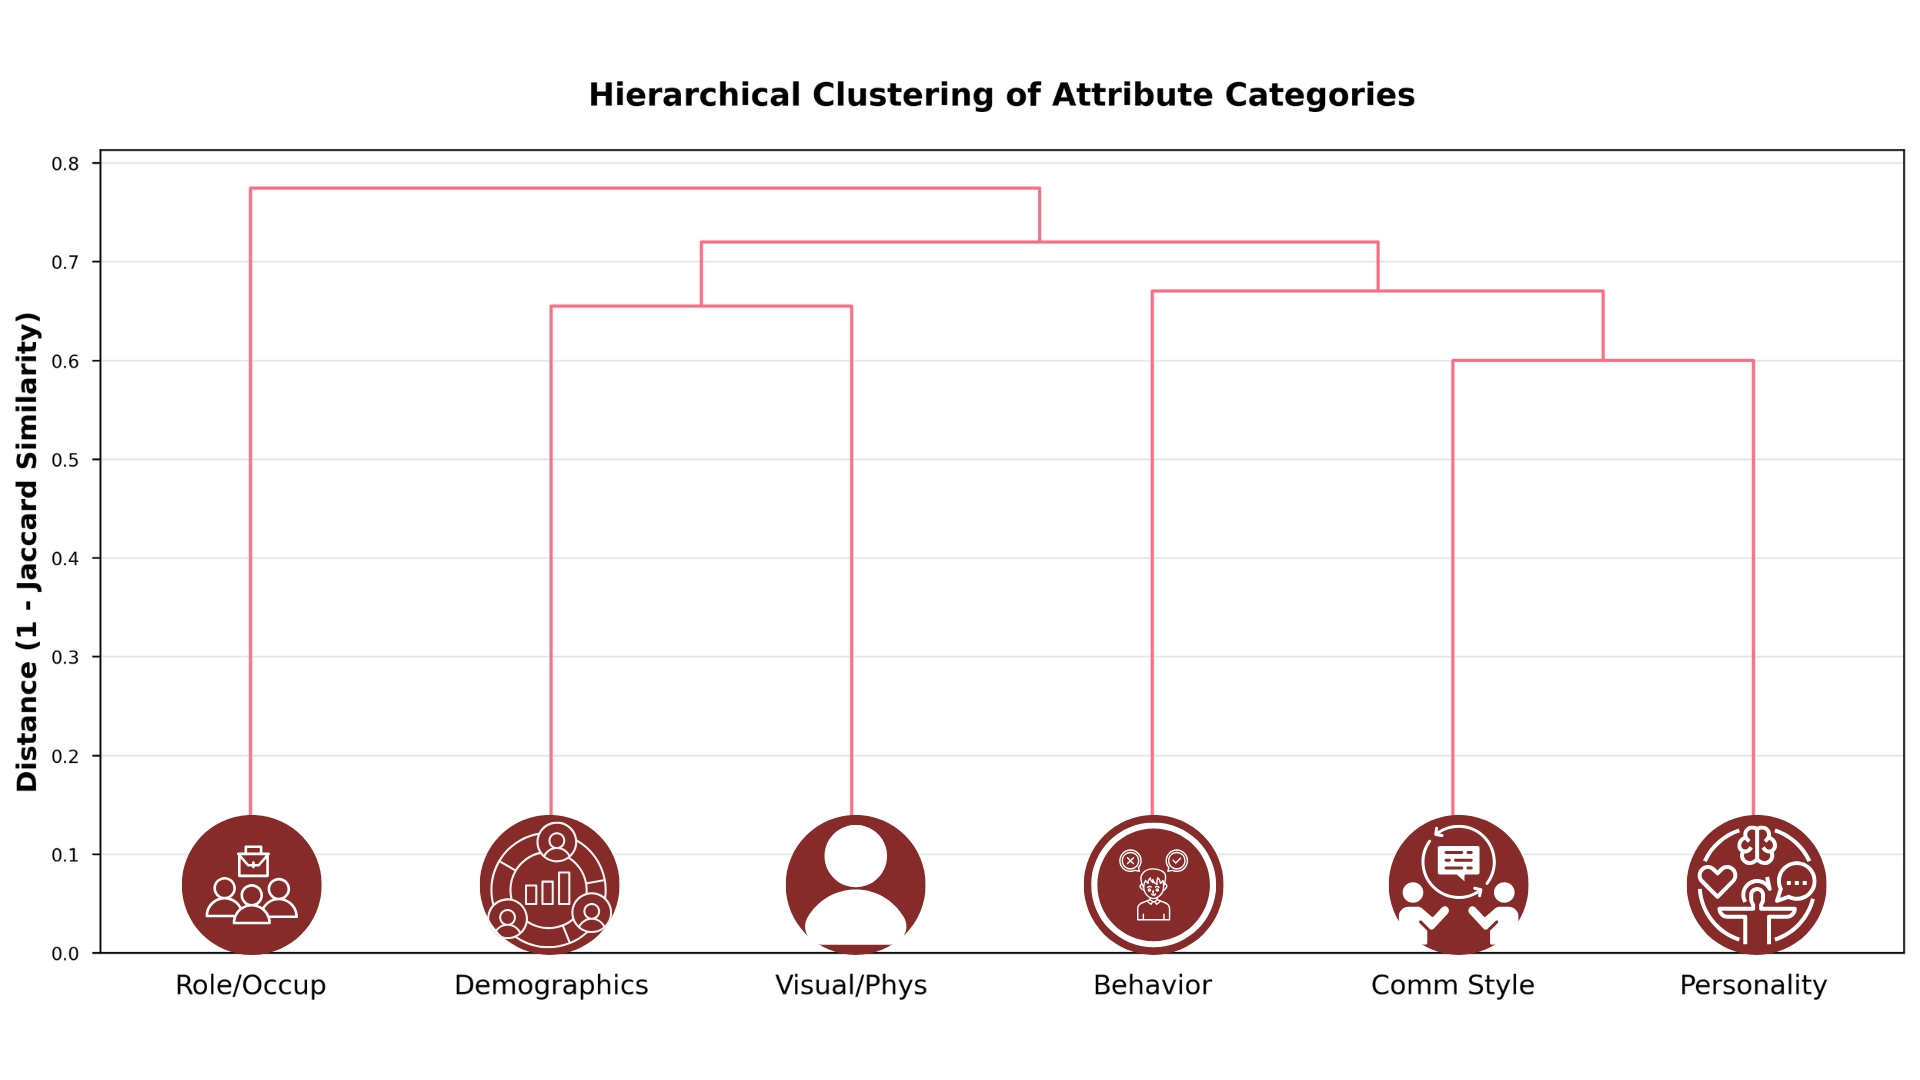
\includegraphics[width=0.7\linewidth]{Figures/clustering_dendogram_b.jpg}
    \caption{\textbf{Clusters of anthropomorphic design in conversational agents.} The dendrogram reveals two primary clusters: a behavioral cluster comprising communication style, personality traits, and behavioral patterns (which group closely together), and an identity cluster including demographic attributes, role/occupation, and visual/physical appearance.}
    \label{fig:dendrogram}
\end{figure}

\begin{table}[htbp]
\centering
\small
\caption{\textbf{Jaccard similarity coefficients for anthropomorphic attribute categories.} Note: *p $<$ .05 based on chi-square test of independence.}
\label{tab:jcc_similarity}
\begin{tabular}{lcccccc}
\hline
\textbf{Category} &
\textbf{CS} &
\textbf{PT} &
\textbf{DA} &
\textbf{BP} &
\textbf{RO} &
\textbf{VPA} \\
\hline
Communication Style (CS) & 1.00 &      &      &      &      &      \\
Personality Traits (PT)  & 0.40 & 1.00 &      &      &      &      \\
Demographic Attributes (DA) & 0.37 & 0.31 & 1.00 &      &      &      \\
Behavioral Patterns (BP) & 0.34 & 0.32 & 0.30 & 1.00 &      &      \\
Role/Occupation (RO) & 0.22 & 0.28 & 0.25 & 0.20 & 1.00 &      \\
Visual/Physical Appearance (VPA) & 0.26 & 0.22 & \textbf{0.34*} & 0.21 & 0.18 & 1.00 \\
\hline
\end{tabular}
\end{table}

\begin{table*}[t]
\centering
\caption{\textbf{Distribution of anthropomorphic attribute categories in 58 anthropomorphization studies.} Behavioral anthropomorphization is more frequent. \textit{Note: The percentages do not sum to 100\% because studies could use multiple categories.}}
\label{tab:attr-dist}
\begin{tabularx}{\textwidth}{@{}llccX@{}}
\toprule
\textbf{Supercategory} & \textbf{Category} & \textbf{n} & \textbf{\%} & \textbf{Attributes Applied} \\
\midrule
\multirow{3}{*}{\shortstack[l]{Behavioral\\attributes\\(n = 76, 65.5\%)}} & Communication style & 29 & 50.0 & conversational (n = 8), polite (n = 2), professional (n = 2) \\
& Personality traits & 28 & 48.3 & empathetic (n = 4), helpful (n = 3), supportive (n = 3) \\
& Behavioral patterns & 19 & 32.8 & proactive (n = 2), initiative-taking (n = 2), engaging \\
\midrule
\multirow{3}{*}{\shortstack[l]{Representational\\attributes\\(n = 45, 38.8\%)}} & Demographic attributes & 22 & 37.9 & gender (n = 11), age (n = 5), cultural background \\
& Role/occupation & 14 & 24.1 & expert (n = 1), personal assistant (n = 1), tutor (n = 1) \\
& Visual/physical appearance & 9 & 15.5 & character (n = 1), facial covering (n = 1), embodiment \\
\bottomrule
\end{tabularx}
\end{table*}


\end{document}